\section{Podstawowe własności szeregów i transformat Fouriera}
%%%%%%%%%%%%%%%%
\begin{frame}[allowframebreaks]{Sposoby opisu procesu fizycznego}
	\begin{enumerate}
		\item w dziedzinie czasu (time domain) $ \implies A(t) $ \\
		$ t - \text{czas}, \quad A - \text{pewna wielkość} $
		%%%%%%%%%%%%%%%%
		\item w dziedzinie: $
		\begin{rcases*}
		\begin{array}{l}
		\text{częstości} (\omega) \\ \text{częstotliwości} (f)
		\end{array}
		\end{rcases*}$
		$\implies \widehat{A}(\omega) \quad \omega = 2 \pi f$
	\end{enumerate}
	$A(t), \quad \widehat{A}(\omega) \,\, - $ dwie różne reprezentacje tej samej funkcji (wielkości fizycznej) związane równaniami transformat Fouriera:
	%%%%%%%%%%%%%%%%
	\begin{block}
	\centering
	\renewcommand{\arraystretch}{1.5}
	\setlength{\abovedisplayskip}{0pt}
	\setlength{\belowdisplayskip}{0pt}
	\setlength{\abovedisplayshortskip}{0pt}
	\setlength{\belowdisplayshortskip}{0pt}
	\[
	\begin{rcases*}
		A(t) = \int\limits_{-\infty}^{\infty}\frac{d \omega}{2\pi}\widehat{A}(\omega) \cdot e^{i \omega t} \\
		\widehat{A}(\omega) = \int\limits_{-\infty}^{\infty}dt \cdot A(t) \cdot e^{-i \omega t}
	\end{rcases*}
	\]
	\end{block}
	lub równoważnie:
	\begin{block}
	\centering
	\renewcommand{\arraystretch}{1.5}
	\setlength{\abovedisplayskip}{0pt}
	\setlength{\belowdisplayskip}{0pt}
	\setlength{\abovedisplayshortskip}{0pt}
	\setlength{\belowdisplayshortskip}{0pt}
	\[
	\begin{rcases*}
		A(t) = \int\limits_{-\infty}^{\infty}df \cdot \widehat{A}(f) \cdot e^{2 \pi ift} \\
		\widehat{A}(f) = \int\limits_{-\infty}^{\infty}dt \cdot A(t) \cdot e^{-2 \pi ift}
	\end{rcases*}
	\begin{array}{r}
		\rightarrow \,\, \text{korzystamy z: } \omega = 2 \pi f\\ \text{nie trzeba pamiętać}\\ \text{o czynniku } \frac{1}{2 \pi}
	\end{array}
	\]
	\end{block}
	$t - \text{czas} \rightleftharpoons \omega - \text{częstość kołowa}$
	\\ $x - \text{położenie} \rightleftharpoons k = \frac{2 \pi}{\lambda} - \text{wektor falowy (liczba falowa)}$
	\\ $\vdots$
	\\ $A(t), \quad \widehat{A}(\omega) \,\, - $ ciągłe f. swych argumentów
	\[
		A(t) \rightleftharpoons \widehat{A}(\omega); \widehat{A}(\omega) = \Gamma[A(t)]
	\]
\end{frame}
%%%%%%%%%%%%%%%%
\begin{frame}{Definicje transformat Fouriera I}
	\begin{enumerate}[a)]
		\item FT - transformata Fouriera (Fourier Transform) \\
		$x$ - ciągłe \\
		$k$ - ciągłe \\
		$A(x), \widehat{A}(k)$ - f. ciągłe
        \begin{columns}
            \begin{column}{0.35\textwidth}
                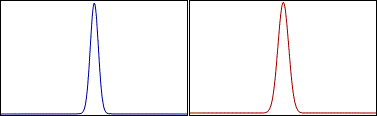
\includegraphics[width=\textwidth]{img/16/ft_wykres1.png}
            \end{column}
            \begin{column}{0.65\textwidth}
                \begin{block}
                    \centering
                    \renewcommand{\arraystretch}{1.5}
                    \setlength{\abovedisplayskip}{0pt}
                    \setlength{\belowdisplayskip}{0pt}
                    \setlength{\abovedisplayshortskip}{0pt}
                    \setlength{\belowdisplayshortskip}{0pt}
                    \[
                        \begin{array}{c}
                            \widehat{A}(k) = \int\limits_{-\infty}^{\infty}dx A(x) e^{-ikx} \\
                            A(x) = \int\limits_{-\infty}^{\infty} \frac{dk}{2 \pi} \widehat{A}(k) e^{ikx}
                        \end{array}
                        \tag{16.1}
                    \]
                \end{block}
            \end{column}
        \end{columns}
	\end{enumerate}
\end{frame}
%%%%%%%%%%%%%%%%
\begin{frame}{Definicje transformat Fouriera II}
	\begin{enumerate}[b)]
		\item FS(i) - szereg Fouriera (Fourier Series) \\
		$x$ - zmienna ciągła \\
		$B(x)$ - f. okresowa ciągłej zmiennej x; okres: L
		\begin{center}
			(ciągła odcinkami wraz z pochodną: na tych odcinkach - szereg zbieżny do B(x), w punktach nieciągłości - do wartości średniej)
		\end{center}
        \begin{columns}
            \begin{column}{0.35\textwidth}
                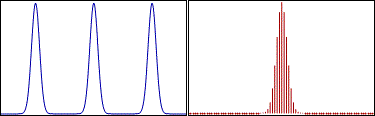
\includegraphics[width=\textwidth]{img/16/fs_wykres1.png}
            \end{column}
            \begin{column}{0.65\textwidth}
                \begin{block}
                    \centering
                    \renewcommand{\arraystretch}{1.5}
                    \setlength{\abovedisplayskip}{0pt}
                    \setlength{\belowdisplayskip}{0pt}
                    \setlength{\abovedisplayshortskip}{0pt}
                    \setlength{\belowdisplayshortskip}{0pt}
                    \[
                        \begin{array}{c}
                            \widehat{B}(k) = \int\limits_{L}dx B(x) e^{-ikx} \\
                            B(x) = \frac{1}{L}\sum\limits_{l = -\infty}^{\infty} \widehat{B}(k) e^{ikx}
                        \end{array}
                        \tag{16.2}
                    \]
                \end{block}
            \end{column}
        \end{columns}
		\begin{tabular}{ll}
			$l$ & - liczba całkowita \\
			$k$ & - dyskretne
		\end{tabular}
		\hfill $k = \underbrace{\frac{2 \pi}{L}}_{k_0} \cdot l = k_0 \cdot l$
	\end{enumerate}
\end{frame}
%%%%%%%%%%%%%%%%
\begin{frame}{Definicje transformat Fouriera III}
	\begin{enumerate}[c)]
		\item FS(ii) - szereg Fouriera \\
		$x_p$ - dyskretne o skoku H \\
		$x_p = p \cdot H$ \\
		$p$ - liczba całkowita
        \begin{columns}
            \begin{column}{0.35\textwidth}
                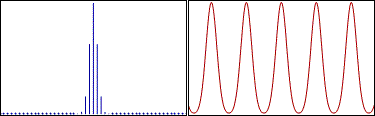
\includegraphics[width=\textwidth]{img/16/dtft_wykres1.png}
            \end{column}
            \begin{column}{0.65\textwidth}
                \begin{block}
                    \centering
                    \renewcommand{\arraystretch}{1.5}
                    \setlength{\abovedisplayskip}{0pt}
                    \setlength{\belowdisplayskip}{0pt}
                    \setlength{\abovedisplayshortskip}{0pt}
                    \setlength{\belowdisplayshortskip}{0pt}
                    \[
                        \begin{array}{c}
                            \widehat{C}(k) = H \cdot \sum\limits_{p = -\infty}^{\infty} C(x_p) e^{-ikx_p} \\
                            C(x_p) = \int\limits_{k_g} \frac{dk}{2 \pi} \widehat{C}(k) e^{ikx_p}
                        \end{array}
                        \tag{16.3}
                    \]
                \end{block}
            \end{column}
        \end{columns}
		$k$ - ciągła \\
		$\widehat{C}(k)$ - periodyczna \\
		okres $k_g = \frac{2 \pi}{H}$
	\end{enumerate}
\end{frame}
%%%%%%%%%%%%%%%%
\begin{frame}{Definicje transformat Fouriera IV}
	\begin{enumerate}[d)]
		\item fFT - skończona transformata Fouriera (finite FT) \\
		$x_p$ - dyskretne o skoku H \\
		$x_p = p \cdot H$ \\
		$D(x_p)$ - okresowa; okres: L \\
		$N$ - ilość punktów w okresie $D(x_p)$ \\
		$k$ - dyskretna, skok $k_0 = \frac{2 \pi}{L}; k = l \cdot k_0$ \\
		$\widehat{D}(k)$ - okresowa, okres $k_g = \frac{2 \pi}{H}$
		\begin{columns}
            \begin{column}{0.35\textwidth}
                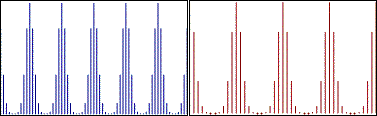
\includegraphics[width=\textwidth]{img/16/dft_wykres1.png}
            \end{column}
            \begin{column}{0.65\textwidth}
                \begin{block}
                    \centering
                    \renewcommand{\arraystretch}{1.5}
                    \setlength{\abovedisplayskip}{0pt}
                    \setlength{\belowdisplayskip}{0pt}
                    \setlength{\abovedisplayshortskip}{0pt}
                    \setlength{\belowdisplayshortskip}{0pt}
                    \[
                        \begin{array}{c}
                        \widehat{D}(k) = H \cdot \sum\limits_{p = 0}^{N-1} D(x_p) e^{-ikx_p} \\
                        D(x_p) = \frac{1}{L} \sum\limits_{l = 0}^{N-1} \widehat{D}(k) e^{ikx_p}
                        \end{array}
                        \tag{16.4}
                    \]
                \end{block}
			\end{column}
		\end{columns}
	\end{enumerate}
\end{frame}
%%%%%%%%%%%%%%%%
\begin{frame}{Związki między transformatami Fouriera}
	Przez przejścia graniczne:\\
	\centering
	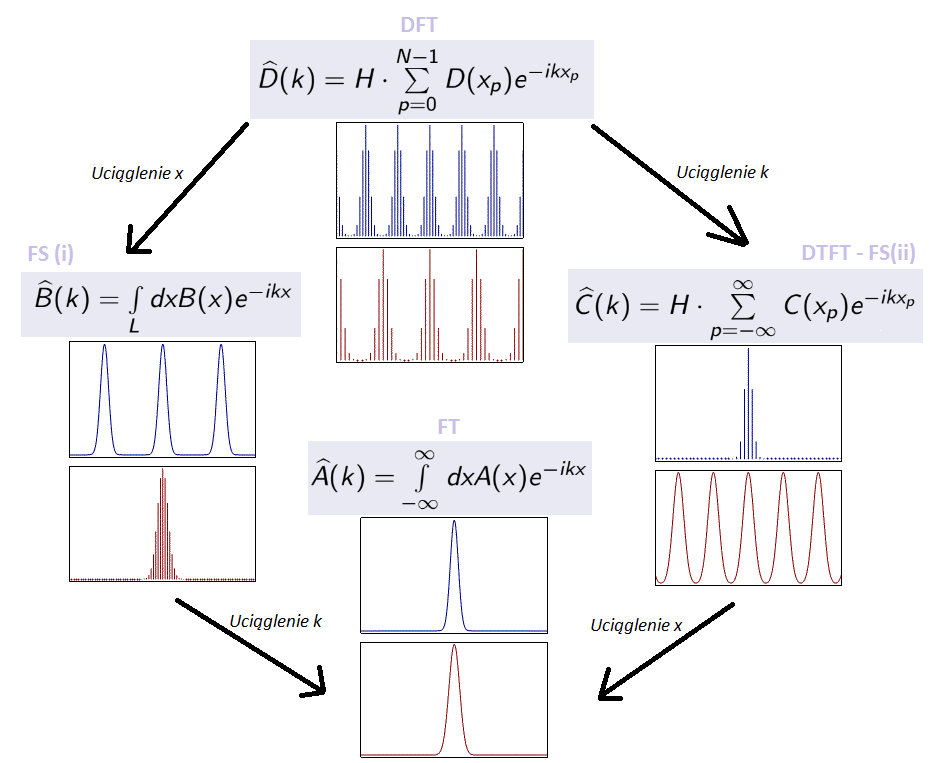
\includegraphics[height=0.8\textheight]{img/16/przejscia_graniczne.png}
\end{frame}
%%%%%%%%%%%%%%%%
\begin{frame}{Symetrie funkcji i jej transformaty I}
	Transformaty Fouriera $\to$ liniowe
	\\ Oznaczenia:
	\begin{itemize}
		\item E - even (parzysty)
		\item O - odd (nieparzysty)
		\item r - real (rzeczywisty)
		\item i - imaginary (urojony)
	\end{itemize}
	Wszystkie 4 transformaty Fouriera mają te same własności symetrii:
	\begin{align*}
		f(x) = E_r(x) + i \cdot E_i(x) + O_r(x) + i \cdot O_i(x) 
		\tag{16.5} \\
		\widehat{f}(k) = E_r(k) + i \cdot E_i(k) + i \cdot O_i(k) + O_r(k)
		\tag{16.6}
	\end{align*}
\end{frame}
%%%%%%%%%%%%%%%%
\begin{frame}{Symetrie funkcji i jej transformaty II}
	\begin{table}
		\centering
		\begin{tabular}{|c|c|}
			\hline
			$f(x)$ & $\widehat{f}(k)$ \\
			\hline
			\hline
			$r \land E$ & $r \land E$ \\
			\hline
			$r \land E$ & $i \land E$ \\
			\hline
			$i \land E$ & $i \land E$ \\
			\hline
			$i \land E$ & $r \land E$ \\
			\hline
			$r$ & hermitowska \\
			\hline
			$i$ & antyherminowska \\
			\hline
			$E$ & $E$ \\
			\hline
			$O$ & $O$ \\
			\hline
		\end{tabular}
	\end{table}
\end{frame}
%%%%%%%%%%%%%%%%
\begin{frame}[allowframebreaks]{Zestawienie własności transformat}
	poza własnościami dotyczącymi pochodnej - obowiązują dla wszystkich 4 transformat \\
	$Z: f(x) \rightleftharpoons \widehat{f}(k); \quad g(x) \rightleftharpoons \widehat{g}(k)$
	\begin{block}
		\centering
		\renewcommand{\arraystretch}{1.5}
		\setlength{\abovedisplayskip}{0pt}
		\setlength{\belowdisplayskip}{0pt}
		\setlength{\abovedisplayshortskip}{0pt}
		\setlength{\belowdisplayshortskip}{0pt}
		\[
		\tag{16.7}
		\begin{array}{@{}ll}
			\text{podobieństwo:} & f(\frac{x}{a}) \rightleftharpoons |a| \cdot \widehat{f}(k \cdot a) \\
			\text{mnożenie przez stałą:} & b \cdot f \rightleftharpoons b \cdot \widehat{f} \\
			\text{suma:} & f + g \rightleftharpoons \widehat{f} + \widehat{g} \\
			\text{odwrotność:} &
			\renewcommand{\arraystretch}{1}
			\begin{array}{@{}l}
				\text{jeżeli:} \quad f(x) \rightleftharpoons \widehat{f}(k) = g(k) \\
				\text{to:} \quad g(x) \rightleftharpoons \widehat{g}(k) = 2 \pi \cdot f(-k)
			\end{array} \\
			\text{przesunięcie:} & f(x + a) \rightleftharpoons e^{ika} \cdot \widehat{f}(k) \\
			\text{pochodna:} & \frac{df}{dx} \rightleftharpoons ik \cdot \widehat{f}(k)
		\end{array}
		\]
	\end{block}
	\begin{theorem}[o mocy]
		\[
			\int\limits_{-\infty}^{\infty} f(x) \cdot g^*(x) dx = \int\limits_{-\infty}^{\infty} \widehat{f}(x) \cdot \widehat{g}^*(x)  \frac{dk}{2 \pi}
			\tag{16.8}
		\]
	\end{theorem}
	Analogicznie dla FS i fFT
\end{frame}
%%%%%%%%%%%%%%%%
\begin{frame}[allowframebreaks]{Splot (konwolucja)}
	$f(x), g(x) -$ funkcje
	$\newline$ \quad ich splot:
	\begin{block}
	\centering
	\renewcommand{\arraystretch}{1.5}
	\setlength{\abovedisplayskip}{0pt}
	\setlength{\belowdisplayskip}{0pt}
	\setlength{\abovedisplayshortskip}{0pt}
	\setlength{\belowdisplayshortskip}{0pt}
	\[
		h(x) = \int\limits_{- \infty}^{\infty} dx' f(x')g(x-x')\equiv f \ast g
		\tag{16.9}
	\]
	\end{block}
	Własności:
	\begin{table}[t]
		\centering
		\begin{tabular}{|c|l|}
			\hline
			$f \ast g = g \ast f$ & commutative \\
			\hline
			$f \ast (g \ast h) = (f \ast g) \ast h$ & associative \\
			\hline
			$f \ast (g +h ) = f \ast g + f \ast h$ & distributive \\
			\hline
		\end{tabular}
	\end{table}
	%%%%%%%%%%%%%%%%
	Przykład operacji splotu dla dwóch wektorów kolumnowych:
	$a \in I\!R^{n\times 1} \ ;\ $ $b \in I\!R^{n\times 1} \ ;\ $
	$a=\begin{bmatrix}
    		\alpha_0 \\
    		\alpha_1 \\
    		\vdots \\
   			 \alpha_{n-1}
		\end{bmatrix}$ ; \quad 
	$b=\begin{bmatrix}
    		\beta_0 \\
    		\beta_1 \\
    		\vdots \\
   			 \beta_{n-1}
		\end{bmatrix}$	
	$
		[ a * b ]_{k} = \sum_{i=0}^{k}\alpha_i \cdot \beta_{k-i};
	$\quad $a * b \in I\!R^{2n\times 1} $\quad
	
	\begin{table}[t]
		\centering
		\scalebox{0.85}{
		\begin{tabular}{ccc}
			 & $\begin{bmatrix} 
    		\beta_{n-1} \\
    		\vdots \\
    		\beta_1 \\
   			 \beta_{0}
			\end{bmatrix}$ & $\bigg\downarrow$ \\
			
			$\begin{bmatrix}
    		\alpha_0 \\
    		\alpha_1 \\
    		\vdots \\
   			 \alpha_{n-1}
			\end{bmatrix}$ &  &  \\ 
			
		\end{tabular}}
		\quad
		\scalebox{0.85}{
		\begin{tabular}{ccc}
		$\Rightarrow$&$ a * b  =$&$\begin{bmatrix} 
    											\alpha_{0} \beta_{0} \\
    											\alpha_{0} \beta_{1} + \alpha_{1} \beta_{0} \\
    											\alpha_{0} \beta_{2} + \alpha_{1} \beta_{1} + \alpha_{2} \beta_{0} \\
    											\vdots \\
    											\alpha_{n-2} \beta_{n-1} + \alpha_{n-1} \beta_{n-2} \\
    											\alpha_{n-1} \beta_{n-1} \\
   			 									0 
												\end{bmatrix}$ \\
		\end{tabular}}
	\end{table}
	
	%%%%%%%%%%%%%%%%
	\begin{table}[t]
	\centering
	\captionsetup{belowskip=-10pt,aboveskip=-10pt}
	\caption{Splot i jego transformaty (16.10)}
		\begin{tabular}{l|l|l}
			& x & k \\
			\hline
				FT
				&
				\begin{tabular}{@{}l}
					$\int\limits_{-\infty}^{\infty} dx' \cdot f(x') \cdot  g(x-x')$ \\
					$f(x) \cdot g(x)$
				\end{tabular}
				&
				\begin{tabular}{@{}l}
					$\widehat{f}(k) \cdot \widehat{g}(k)$ \\
					$\int\limits_{-\infty}^{\infty} \frac{dk'}{2 \pi} \cdot \widehat{f}(k') \cdot \widehat{g}(k - k')$
				\end{tabular} \\
			\hline
				FS(i)
				&
				\begin{tabular}{@{}l}
					$\int\limits_{L} dx' \cdot f(x') \cdot g(x - x')$ \\
					$f(x) \cdot g(x)$
				\end{tabular}
				&
				\begin{tabular}{@{}l}
					$\widehat{f}(k) \cdot \widehat{g}(k)$ \\
					$\frac{1}{L} \cdot \sum\limits_{L' = -\infty}^{\infty} \widehat{f}(k') \cdot \widehat{g}(k - k')$
				\end{tabular} \\
			\hline
				FS(ii)
				&
				\begin{tabular}{@{}l}
					$H \cdot \sum\limits_{p' = -\infty}^{\infty}  f(x'_p) \cdot g(x_p - x'_p)$ \\
					$f(x_p) \cdot g(x_p)$
				\end{tabular}
				&
				\begin{tabular}{@{}l}
					$\widehat{f}(k) \cdot \widehat{g}(k)$ \\
					$\int\limits_{k_g} \frac{dk'}{2 \pi} \cdot  \widehat{f}(k') \cdot \widehat{g}(k - k')$
				\end{tabular} \\
			\hline
				fFT
				&
				\begin{tabular}{@{}l}
					$H \cdot \sum\limits_{p' = 0}^{\infty} f(x'_p) \cdot  g(x_p - x'_p)$ \\
					$f(x_p) \cdot g(x_p)$
				\end{tabular}
				&
				\begin{tabular}{@{}l}
					$\widehat{f}(k) \cdot \widehat{g}(k)$ \\
					$\frac{1}{l} \cdot \sum\limits_{l' = 0}^{N - 1}  \widehat{f}(k') \cdot \widehat{g}(k - k')$
				\end{tabular}
		\end{tabular}
	\end{table}
\end{frame}
%%%%%%%%%%%%%%%%
\begin{frame}{Transformaty 3-D i \dots}
	Uogólnienie z 1-D na 3-D (i więcej) - bezpośrednie:
	\begin{table}[t]
		\centering
		\renewcommand{\arraystretch}{1.35}
		\[
		\tag{16.11}
		\begin{array}{c|l}
			\text{1-D} & \text{3-D} \\
			\hline
			x & \vec{x} = (x_1, x_2, x_3) \\
			k & \vec{k} = (k_1, k_2, k_3) \\
			k\cdot x & \vec{k} \cdot \vec{x} \\
			dx & d\vec{x} \\
			\frac{d\vec{k}}{2\pi} & \frac{dk}{(2\pi)^3} \\
			L & V_b = L_1 \cdot L_2 \cdot L_3 \\
			H & V_c = H_1 \cdot H_2 \cdot H_3 \\
			& \dots
		\end{array}
		\]
		\renewcommand{\arraystretch}{1}
	\end{table}
\end{frame}